\documentclass[runningheads]{llncs}
\usepackage{graphicx}
\usepackage{amsmath,amssymb} % define this before the line numbering.
\usepackage{ruler}
\usepackage{color}
\usepackage{censor}

%===========================================================
% Custom commands
\newcommand{\mat}{\mathbf}
\DeclareMathOperator{\pa}{pa}
\DeclareMathOperator{\argmin}{arg min}

%===========================================================
\begin{document}
\pagestyle{headings}
\mainmatter{}

\def\ACCV16SubNumber{***}  % Insert your submission number here

%===========================================================
\title{Exploiting Temporal Relationships for Human Pose Estimation using Biposelets}
\titlerunning{ACCV-16 submission ID \ACCV16SubNumber}
\authorrunning{ACCV-16 submission ID \ACCV16SubNumber}

\author{Anonymous ACCV 2016 submission}
\institute{Paper ID \ACCV16SubNumber}

\maketitle

%%%%%%%%%%%%%%%%%%%%%%%%%%%%%%%%%%%%%%%%%%%%%%%%%%%%%%%%%%%%%%%%%%%%%%%%%%%%%%%
% Misc formatting notes:
%
% - Use "This is not a pipe~\cite{sourceYY}." to cite papers (not fancy natbib
%   stuff)
% - They want punctuated equations and a ~ space between the end of the equation
%   and the punctuation (either comma or full stop).
% - Don't feel obligated to go to 14 pages. A quick skim of accepted papers from
%   ACCV 2014 shows that going above 10 pages is the norm (shortest I saw was 12
%   pages), but that fewer than 14 pages of actual content is totally
%   acceptable.
% - Structure is flexible. For instance:
%   - There's no need for a separate discussion section (apart from discussion
%     in experiments section)
%   - Some authors don't include a separate section for related work, some do.
%   - Long sections are acceptable (but poor practice, IMO)

%%%%%%%%%%%%%%%%%%%%%%%%%%%%%%%%%%%%%%%%%%%%%%%%%%%%%%%%%%%%%%%%%%%%%%%%%%%%%%%
% Tentative list of figures to produce:
%
% - One flow chart for the entire pose estimation process (re-use images from
%   PowerPoint, but in Inkscape or something that plays nicely with LaTeX)
% - Big panel of biposelets
% - Illustration of stitching model for single frames (much like the one in my
%   PowerPoint)
% - Panels of good at bad predictions for MPII Cooking Activities, Poses in the
%   Wild and H3.6M
% - Possibly a small summary figure at the beginning showing some representative
%   detections to lend flavour to the rest of the paper.
% - Possibly CNN architecture diagram showing how flow is merged with RGB
%   images---would prefer not to do that, since it's not a well-explored aspect
%   of my approach.
% - Plots of PCK and strict PCP:
%   - Raw PCK for Poses in the Wild
%   - PCP-strict at various thresholds for PIW (include table for PCP@0.5)
%   - PCP-strict at various thresholds for MPII Cooking Activities (also needs
%     table for PCP@0.5)
%   - PCKh for H3.6M in same format as recurrent convnet paper

%%%%%%%%%%%%%%%%%%%%%%%%%%%%%%%%%%%%%%%%%%%%%%%%%%%%%%%%%%%%%%%%%%%%%%%%%%%%%%%
% Page budgeting (14 page content limit with unlimited references):
%
% - 1 page for introduction, abstract and title
% - 1-2 pages for related work
% - 4-5 pages for method (frame pair model + stitching + learning)
% - 5-6 pages for experiments and discussion (depending on space available)
% - 0.5 pages for conclusion and acknowledgement

\begin{abstract}
The problem of human pose estimation in still images has been well-studied in
recent years, but making effective use of the temporal information inherent in
videos is still an open problem. We propose a new model which attempts to learn
temporal relationships by using a CNN to predict poses for several frames at a
time; our model caters to the detection capabilities of CNNs by casting pose
estimation as a problem of predicting the \textit{biposelets} which poses in
adjacent frames are composed of. Predicting poses in two frames at a time
reduces pose estimation over an entire video sequence to the problem of choosing
a pose for each frame from a set of high-scoring poses, which can be achieved by
minimising a trivial pairwise cost with dynamic programming. Experiments show
that our approach performs competitively with existing approaches on established
pose estimation benchmarks.
\end{abstract}

\section{Introduction}

% Things I want to say:
% Why pose estimation in general is interesting:
%  - Challenging task in general
%  - Use it for 3D pose estimation
%  - Use it for action recognition (P-CNN paper is relevant example)
%  - Use it for just about everything else
% Why video pose estimation in particular is interesting:
%  - Few results so far
%  - Intuitively seems like temporal information should lead to big improvement
%  - Hard to actually get solid improvement in practice
% How we approach the problem; briefly summarise the biposelet detection and
% sequence stitching stages here.
% Our results

\section{Related work}

% Work I want to mention:
% Some papers on poselets
% Xianjie Chen's stuff (graphical models!)
% Toshev & Szegedy (CNNs)
% Modeep
% Convolutional pose machines
% Anoop's stuff
% Flowing convnets
% "Recurrent human dynamics paper" (poor results, interesting approach)

\section{Detecting pose pairs}

% What I want to say:
% - Objective of this stage of pipeline is to find a pose in each frame of each
%   neighbouring frame pair.
% - Decompose pose into several subposes.
% - Intuitively: want to predict a configuration (poselet) for each subpose.
%   Choose configurations by applying K-means to all relative positions. This is
%   tied to the CNN training step, so I will have to explain it there.
% - In our method: each configuration gives a location for each joint within
%   both frames. This allows configurations to capture both location and motion.
%   Call these configurations biposelets.
% - NOW talk about cost function.
% - Talk about pairwise costs and how the means are found for the pairwise
%   costs.
% - Need to mention optical flow implementation in use
% - Talk about maximising cost function.
%   - Just message passing with distance transforms.
%   - Need complexity mentioned in there somewhere.
% - How unaries are produced and learnt by CNN (one follows from the other):
%   - CNN architecture
%   - CNN input (two frames + flow between them)
%   - CNN output
%   - CNN objective.
%   - Fully convolutional inference
%   - Learning (just SGD) --> maybe put the training details in the experiments
%     section.
% - How SSVM is learnt. Talk about learning target, how positives/negatives are
%   used, where supervision comes in (if anywhere), how things are optimised
%   (just cite ramanan2013dual). <-- Maybe put in learning section
% - How poses are recovered from a set of subpose locations and types for each
%   subpose.

\subsection{Subposes and biposelets}\label{sec:decomp}

In the first stage of our pipeline, we consider each neighbouring pair of frames
in a sequence and simultaneously infer the poses present in each. For the
purposes of this stage, we decompose a pair of poses in neighbouring frames into
a fixed set of subposes, each of which correspond to a subset of joints in the
original pose. Subposes are chosen so that each subpose shares exactly a joint
with at least one neighbouring subpose, and each joint in the original pose is
present in at least one subpose. For instance, a pose containing shoulder, elbow
and wrist joints could be decomposed into one subpose containing wrist and elbow
joints on the left side of the body, one subpose containing elbow and shoulder
joints on the left hand side, one subpose containing both the left and right
shoulders, etc.

Rather than representing the locations of each joint in each subpose directly,
we discretise the space of configurations for joints within each subpose into
$K$ \textit{biposelets}. Biposelets are so named in analogy to the
\textit{poselets} of Bourdev and Malik~\cite{bourdev2009poselets}. Unlike their
namesake, however, biposelets give a position for each joint in a subpose across
two video frames instead of a single one. This allows biposelets to represent
both the relative positions of joints and their movement over time. A
representative set of biposelets learnt for the MPII Cooking Activities pose
estimation dataset~\cite{rohrbach2012database} is shown in
Figure~\ref{fig:biposelets}.

\begin{figure*}[t]
\begin{center}
\begin{tabular}{@{}c@{}c@{}c@{}c@{}c@{}c@{}c@{}c@{}}
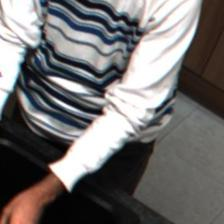
\includegraphics[height=0.1375\linewidth]{figures/biposelets/poselet-230/sample-1-f0.jpg}\,&
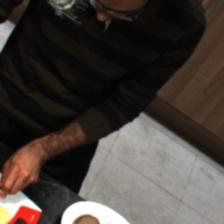
\includegraphics[height=0.1375\linewidth]{figures/biposelets/poselet-230/sample-2-f0.jpg}\,&
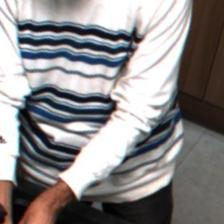
\includegraphics[height=0.1375\linewidth]{figures/biposelets/poselet-230/sample-3-f0.jpg}\,&
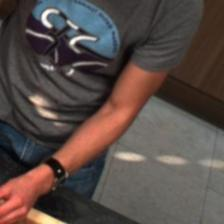
\includegraphics[height=0.1375\linewidth]{figures/biposelets/poselet-230/sample-4-f0.jpg}\,&
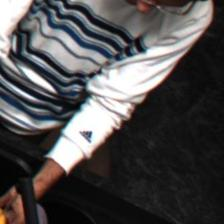
\includegraphics[height=0.1375\linewidth]{figures/biposelets/poselet-230/sample-5-f0.jpg}\,&
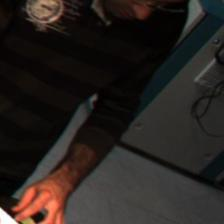
\includegraphics[height=0.1375\linewidth]{figures/biposelets/poselet-230/sample-6-f0.jpg}\,&
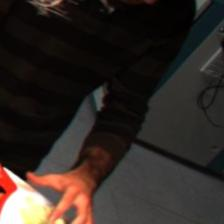
\includegraphics[height=0.1375\linewidth]{figures/biposelets/poselet-230/sample-7-f0.jpg}\\
%
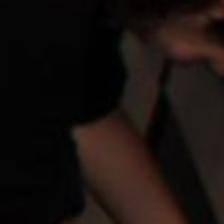
\includegraphics[height=0.1375\linewidth]{figures/biposelets/poselet-289/sample-1-f0.jpg}\,&
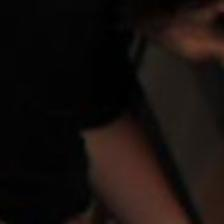
\includegraphics[height=0.1375\linewidth]{figures/biposelets/poselet-289/sample-2-f0.jpg}\,&
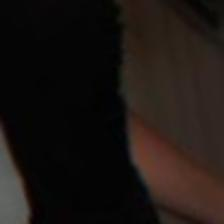
\includegraphics[height=0.1375\linewidth]{figures/biposelets/poselet-289/sample-3-f0.jpg}\,&
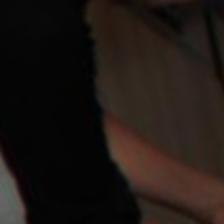
\includegraphics[height=0.1375\linewidth]{figures/biposelets/poselet-289/sample-4-f0.jpg}\,&
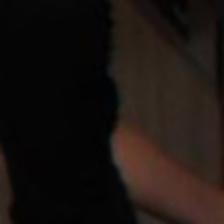
\includegraphics[height=0.1375\linewidth]{figures/biposelets/poselet-289/sample-5-f0.jpg}\,&
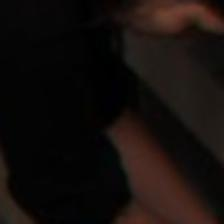
\includegraphics[height=0.1375\linewidth]{figures/biposelets/poselet-289/sample-6-f0.jpg}\,&
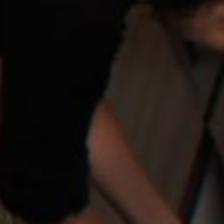
\includegraphics[height=0.1375\linewidth]{figures/biposelets/poselet-289/sample-7-f0.jpg}\\
%
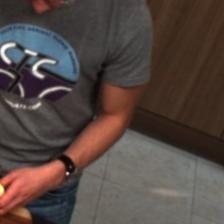
\includegraphics[height=0.1375\linewidth]{figures/biposelets/poselet-297/sample-1-f0.jpg}\,&
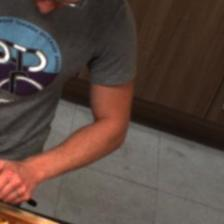
\includegraphics[height=0.1375\linewidth]{figures/biposelets/poselet-297/sample-2-f0.jpg}\,&
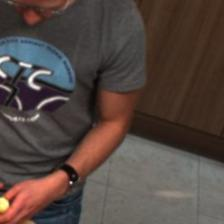
\includegraphics[height=0.1375\linewidth]{figures/biposelets/poselet-297/sample-3-f0.jpg}\,&

\includegraphics[height=0.1375\linewidth]{figures/biposelets/poselet-297/sample-4-f0.jpg}\,&
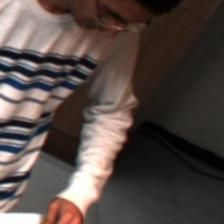
\includegraphics[height=0.1375\linewidth]{figures/biposelets/poselet-297/sample-5-f0.jpg}\,&
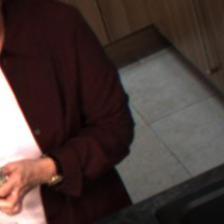
\includegraphics[height=0.1375\linewidth]{figures/biposelets/poselet-297/sample-6-f0.jpg}\,&
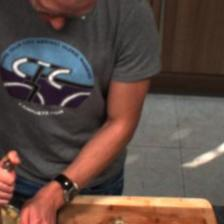
\includegraphics[height=0.1375\linewidth]{figures/biposelets/poselet-297/sample-7-f0.jpg}\\
\end{tabular}
\end{center}
\caption{Biposelets learnt for left elbows in the MPII Cooking Activities
dataset. Different rows show different biposelets. For brevity,
only the first frame associated with each biposelet is shown.}
\label{fig:biposelets}
\end{figure*}

% TODO: Give motivation for decomposing into subposes and biposelets instead of:
% 1) Considering a single joint at a time
% 2) Considering the entire pose

\subsection{Frame pair model}

Formally, our frame pair model conceptualises a pose as a tree-structured graph
$\mathcal G = (\mathcal S, \mathcal E)$ consisting of a set of subposes
$\mathcal S$ and a set of edges $\mathcal E \subset \mathcal S \times \mathcal
S$. Subposes are chosen according to the constraints listed in
Section~\ref{sec:decomp}, and a pair of subposes $(s_1, s_2)$ will have an edge
between them iff they have a joint in common. The objective of the first stage
of our pipeline is to take a pair of frames $(\mat I_1, \mat I_2)$ and output,
for each subpose $s$, a subpose location $\vec l_s \in \mathbb R^2$ within the
frame pair and a biposelet type $t_s \in \{1, \ldots, K\}$. Specifically, the
first stage must find some $\mat L = \begin{bmatrix}\vec l_1 & \vec l_2 & \cdots
& \vec l_{|\mathcal S|}\end{bmatrix}^T$ and $\vec t = \begin{bmatrix}t_1 & t_2 &
\cdots & t_{|\mathcal S|}\end{bmatrix}$ which minimises the cost
%
\begin{equation}\label{eqn:full-cost}
C(\mat L, \vec t \mid \mat D_{12})
= w_0 + \sum_{s \in \mathcal V} \phi_s(\vec l_s, t_s; \mat D_{12})
+ \sum_{(s_1, s_2) \in \mathcal E}
    \psi_{s_1 s_2}(\vec l_{s_1}, \vec l_{s_2}, t_1, t_2),
\end{equation}
%
where $w_0$ is a bias, each $\phi_s(\cdot)$ is an appearance term, each
$\psi_{s_1,s_2}$ is a pairwise cost, and $\mat D_{12}$ is the concatenation
of $\mat I_1$ and $\mat I_2$.

Recall that each pair of neighbouring subposes have a single joint in common;
the aim of the pairwise terms is to ensure that locations of neighbouring
subposes are chosen so that predicted locations for their shared joints are
consistent. Concretely, each pairwise cost can be written out in full as
%
\begin{equation}\label{eqn:pair-cost}
\psi_{s_1 s_2}(\vec l_{s_1}, \vec l_{s_2}, t_1, t_2)
= \langle
    \vec w_{s_1 s_2},
    \vec \Delta(\vec l_{s_1} - \vec l_{s_2}  - \vec m_{t_1 t_2})
\rangle,
\end{equation}
%
where $\vec \Delta(\begin{bmatrix}\delta_x & \delta_y\end{bmatrix}) =
\begin{bmatrix}\delta_x^2 & \delta_x & \delta_y^2 & \delta_y\end{bmatrix}$ is a
deformation feature, $\vec w_{s_1 s_2}$ is a learnt weight vector, and
$\vec m_{t_1 t_2}$ is an ``ideal'' displacement between $s_1$ and $s_2$. %TODO

%TODO
\begin{equation}\label{eqn:unary-cost}
\phi_s(\vec l_s, t_s; \mat D_{12}) = -w_s \log p(s, t_s \mid \mat D_{12}(\vec l_s))
\end{equation}
%
where $w_s$ is a learnt weight and $\mat D_{12}(\vec l_s)$ denotes a crop of the
frame pair $(\mat I_1, I_2)$ and the optical flow between them at location $\vec
l_s$.

\subsection{Computation of appearance terms}
\label{sec:unaries}

% TODO: Describe the CNN used to calculate appearance terms in depth (so inputs,
% outputs, use of fully convolutional network, etc.). Leave learning for the
% learning section, though.

% Inference on a frame pair proceeds in three steps: first, optical flow is
% computed between the two frames using Brox et al.'s
% approach~\cite{brox2004high}.

\subsection{Inference on frame pair model}

The full cost (\ref{eqn:full-cost}) can be minimised efficiently by exploiting
the subpose graph's tree structure. For each subpose $s$, define the minimal
cost of the subtree rooted at $s$ as
%
\begin{equation}\label{eqn:reccost}
\begin{split}
M(\vec l_s, t_s; \mat D_{12}) =
&\sum_{s' : \pa(s') = s} \min_{\vec l_{s'}, t_{s'}} \left(\psi_{s s'}(\vec l_s,
\vec l_{s'}, t_s, t_{s'}) + M(\vec l_{s'}, t_{s'}; \mat D_{12})\right)
\\&\quad+ \phi_s(\vec l_s, t_s; \mat D_{12}),
\end{split}
\end{equation}
%
where $\vec l_s$ and $t_s$ are the location and biposelet type, respectively, of
$s$, and $\pa(s') = s$ iff subpose $s$ is the parent of subpose $s'$ in
$\mathcal G$.

$M$ can be calculated for location and type of the root subpose subpose by
proceeding from the leaves of $\mathcal G$ upwards: for each leaf subpose $s_l$,
$M(\vec l_{s_l}, t_{s_l}; \mat D_{12})$ is simply $\phi_{s_l}(\vec l_{s_l},
t_{s_l}; \mat D_{12})$. For a non-leaf subpose $s$, $M(\vec l_s, \vec t_s; \mat
D_{12})$ can be computed by first evaluating $M(\vec l_{s_c}, t_{s_c}; \mat
D_{12})$ for each child $s_c$ of $s$, then applying Felzenszwalb and
Huttenlocher's distance transform technique~\cite{felzenszwalb2012distance} to
find the $\vec l_{s_c}$ which minimises $\psi_{s s_c}(\vec l_s, \vec l_{s_c},
t_s, t_{s_c})$ for each $t_{s_c}$.

$\mathcal O(N K^2)$ time.
%TODO: Complexity analysis
In a frame pair with $N$ unary map locations, calculating $M$ for all locations
and types of the root subpose takes $\mathcal O(|\mathcal S| N K^2)$ time.

Having evaluated (\ref{eqn:reccost}) for each possible $\vec l_{s_R}$ and
$t_{s_R}$, finding the pose configuration which minimises (\ref{eqn:full-cost})
is a simple matter of looking up
%
\begin{equation}
\argmin_{\vec l_{s_R}, t_{s_R}} M(\vec l_{s_R}, \vec t_{s_R}; \mat D_{12})
\end{equation}
%
and then backtracking to recover the locations
and types of all other subposes. This backtracking process can be repeated for
several root locations and types to produce a set of low-cost pose
configurations for each frame pair; having several such configurations is
important during the sequence stitching stage of the pipeline, as explained in
Section~\ref{sec:stitching}.

\section{Sequence stitching}\label{sec:stitching}

% Things I want to talk about:
%
% - How to go from a sequence of subpose types and locations for each pair to a
%   set of poses for each frame.
% - Sequence stitching cost and cost minimisation (dynamic programming).
% - Why this is an improvement over other methods (fewer parameters, less
%   complicated implementation)

In the second stage of our pipeline, we attempt to produce a temporally coherent
sequence of poses across every frame of a video.%TODO

After determining a location and biposelet type for each subpose, we can recover
a location for each joint in the original pose model%TODO

\section{Learning}

% Things I need to explain:

\subsection{Learning unaries}

% How CNN is learnt (what is the general learning setup? What augmentations do
% we apply? What about SGD parameters?)

\subsection{Clustering biposelets}

% How biposelets are clustered (apply K-means to joints in CNN training patches)

\subsection{Single-pair detector}

% Structural SVM things
\cite{ramanan2013dual}

\subsection{Stitching weights}

% Randomized search on validation set showed that stitching is pretty much
% invariant to order-of-magnitude changes in relative values of variables, so in
% practice you can probably pick coefficients by hand). Need to explain this in
% a way which sounds reasonable sophisticated.

\section{Experiments}

% Things I want to include:
% - Some sort of performance evaluation. Probably just measure eval time on
%   Poses in the Wild, or perhaps time-per-frame-pair for each pair in each of
%   the datasets, then mean recombination time per frame. Over all the test
%   sequences.

% XXX: Remove censor box for camera-ready version
Code for all experiments is available at \censor{\url{https://github.com/qxcv/joint-regressor}}.

\paragraph{MPII Cooking Activities}

% TODO: PCKh graphs (raw PCK given elsewhere, but I can probably ignore that),
% PCP for each limb, qualitative results

% Other papers I will try to use:
% - This paper: http://www.cv-foundation.org/openaccess/content_iccv_2015/papers/Cheron_P-CNN_Pose-Based_CNN_ICCV_2015_paper.pdf
%   ^ Very relevant! Seems to be action recognition paper where they've also
%     tackled pose estimation. Also check out http://jhmdb.is.tue.mpg.de/ (SHIT!)
%   ^ https://github.com/gcheron/P-CNN has a link to computed joint positions
%     over all of MPII cooking activities (!!)
%   ^ Oh wait, they're using Anoop's CVPR '14 paper to compute poses :( At least
%     they show that using the GT poses (which I'll hopefully be closer to)
%     improves performance by double-digits.
% - Project results here into 2D: https://www.mpi-inf.mpg.de/fileadmin/inf/d2/amin/sikandar2013bmvc.pdf
% - Results from here (shitty): https://www.mpi-inf.mpg.de/fileadmin/inf/d2/amin/rohrbach12cvpr.pdf
% - Here: http://link.springer.com/chapter/10.1007/978-3-319-11752-2_20#page-1

\paragraph{FLIC and PIW}

% TODO: PCKh graphs, PCP for each limb, qualitative results

% Other papers I will try to use:
% - Anoop's original paper
% - Xianjie Chen's paper from last year (just collapse my model into Chen &
%   Yuille's model, or maybe use their code but with FLIC stuff)
% - Flowing convnets paper

% Note that I already have (un-normalised results) for each of those sitting on
% Github, and they are comparable with the Flowing Convnets paper
% (http://www.cv-foundation.org/openaccess/content_iccv_2015/papers/Pfister_Flowing_ConvNets_for_ICCV_2015_paper.pdf),
% which also fails to normalise anything.

\paragraph{Human3.6M} Human3.6M~\cite{ionescu2014human,ionescu2011latent} (herein abbreviated as H3.6M)

% TODO: PCKsh (as in shoulder->hip normalised) plots, qualitative results

% Other papers I will try to use:
% - Don't bother with Anoop's code or Xianjie Chen's code! This is a totally
%   alien dataset which will require a LOT of hacking.
% - http://www.cv-foundation.org/openaccess/content_iccv_2015/papers/Fragkiadaki_Recurrent_Network_Models_ICCV_2015_paper.pdf
%   ^ May also be able to use PF and VITERBI baselines
%   ^ Project page at http://www.cs.berkeley.edu/~katef/humandynamics.html but
%     no results or code. WTF :(
%   ^ Can probably rip their results out of their PDF using some sort of hacks.
%     The problem is that the plots are stored as PNG images, which makes it
%     hard to extract their stats *accurately*
% - Cast to 2D: http://www.cv-foundation.org/openaccess/content_cvpr_2014/papers/Ionescu_Iterated_Second-Order_Label_2014_CVPR_paper.pdf
%   ^ There's a project page at http://catalinionescu.weebly.com/label-sensitive-pooling.html
%     but no results to download
% - Cast to 2D: http://ieeexplore.ieee.org/stamp/stamp.jsp?tp=&arnumber=7293666

\section{Conclusion}

\section*{Acknowledgments}

We would like to thank various authors whose code we have extended or used to
produce baseline
comparisons~\cite{pfister2015flowing,chen2014articulated,cherian2014mixing}.

%References are listed in alphabetic order by the surname of the first author, or the identifying word (e.g., in case of a website). Have
%all anonymized references at the beginning of the list.

%here would be your acknowledgement (if any) in the final accepted paper

%===========================================================
\bibliographystyle{splncs}
\bibliography{citations}
\end{document}
